% This is text associated with the open textbook "Open Electromagnetics"
% See immediately below for author, date
% This work is licensed under the Creative Commons Attribution-ShareAlike 4.0 International License. (CC BY-SA 4.0) 
% To view a copy of the license, visit http://creativecommons.org/licenses/by-sa/4.0/

%ORB TITLE Total Internal Reflection
%ORB AUTHOR 0        # S.W. Ellingson, Virginia Tech (ellingson@vt.edu)
%ORB DATE 20191120   # yyyymmdd
%ORB ABSTRACT 

\label{m0169_Total_Internal_Reflection} % <-- Must match name of this file and module directory name.  Don't mess with this!
\index{total internal reflection|(}

\emph{Total internal reflection} refers to a particular condition resulting in the complete reflection of a wave at the boundary between two media, with no power transmitted into the second region.
One way to achieve complete reflection with zero transmission is simply to require the second material to be a perfect conductor.
However, total \emph{internal} reflection is a distinct phenomenon in which neither of the two media are perfect conductors.
Total internal reflection has a number of practical applications; notably, it is the enabling principle of fiber optics.
\index{fiber optics}

Consider the situation shown in Figure~\ref{m0169_fOblique}: 
%
\begin{figure}[b!]
\begin{center}
\pdftooltip{{  % note double braces
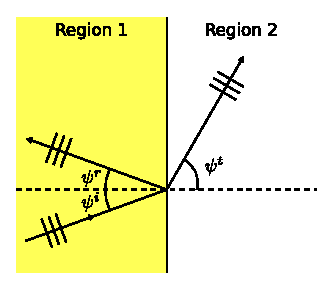
\includegraphics[width=0.8\columnwidth]{modules/m0169_fOblique.eps} 
% https://commons.wikimedia.org/wiki/File:Upw_incident_on_planar_boundary_angle_reflection_equals_incidence.svg
}}{A vertical planar boundary separates region 1 (left) and region 2 (right). The incident plane wave travels through region 1 at an acute angle of small psi superscript i measured to the horizontal. The reflected wave is at an angle small psi superscript r to the horizontal. The transmitted wave is an angle small psi superscript t measured to the vertical.}
\end{center}
\centerline{\scriptsize 
\copyright~\hyperref[m0169_fOblique_Credit]{C.\ Wang} 
\href{https://creativecommons.org/licenses/by-sa/4.0/}{CC BY-SA 4.0} (modified)
} 
\caption{
\label{m0169_fOblique}
A uniform plane wave obliquely incident on the planar boundary between two semi-infinite material regions.
Here $\mu_{r1}\epsilon_{r1}>\mu_{r2}\epsilon_{r2}$, so $\psi^t>\psi^i$.
}
\end{figure}
%
A uniform plane wave is obliquely incident on the planar boundary between two semi-infinite material regions.
In Section~\ref{m0168_Angles_of_Reflection_and_Refraction}, it is found that 
%
\begin{equation}
\psi^r = \psi^i 
\end{equation}
%
i.e., angle of reflection equals angle of incidence.
Also, from Snell's law:
\index{Snell's law}
%
\begin{equation}
\sqrt{\mu_{r1}\epsilon_{r1}} \sin\psi^i = \sqrt{\mu_{r2}\epsilon_{r2}} \sin\psi^t 
\label{m0169_eAt3}
\end{equation}
%
where ``$r$'' in the subscripts indicates the relative (unitless) quantities.
The associated formula for $\psi^t$ explicitly is:
%
\begin{equation}
\psi^t = \arcsin\left(\sqrt{\frac{\mu_{r1}\epsilon_{r1}}{\mu_{r2}\epsilon_{r2}}} \sin\psi^i \right)  
\label{m0169_eAt}
\end{equation}

From Equation~\ref{m0169_eAt}, it is apparent that when $\mu_{r1}\epsilon_{r1}>\mu_{r2}\epsilon_{r2}$, $\psi^t>\psi^r$;
i.e., the transmitted wave appears to bend away from the surface normal, as shown in Figure~\ref{m0169_fOblique}.
In fact, $\psi^t$ can be as large as $\pi/2$ (corresponding to propagation parallel to the boundary) for angles of incidence which are less than $\pi/2$.
What happens if the angle of incidence is further increased?
When calculating $\psi^t$ using Equation~\ref{m0169_eAt}, one finds that 
the argument of the arcsine function becomes greater than 1.
Since the possible values of the sine function are between $-1$ and $+1$, the arcsine function is undefined.
Clearly our analysis is inadequate in this situation.

To make sense of this, let us begin by identifying the threshold angle of incidence $\psi^i_c$ at which the trouble begins.
From the analysis in the previous paragraph,
%
\begin{equation}
\sqrt{\frac{\mu_{r1}\epsilon_{r1}}{\mu_{r2}\epsilon_{r2}}} \sin\psi^i_c = 1
\end{equation}
%
therefore,
%
\begin{equation}
\boxed{
\psi^i_c = \arcsin\sqrt{\frac{\mu_{r2}\epsilon_{r2}}{\mu_{r1}\epsilon_{r1}}}
}
\label{m0169_eCA}
\end{equation}
%
This is known as the \emph{critical angle}.
\index{critical angle}
When $\psi^i<\psi^i_c$, our existing theory applies.
When $\psi^i\ge\psi^i_c$, the situation is, at present, unclear.
For non-magnetic materials, Equation~\ref{m0169_eCA} simplifies to
%
\begin{equation}
\psi^i_c = \arcsin\sqrt{\frac{\epsilon_{r2}}{\epsilon_{r1}}}
\label{m0169_eCAnm}
\end{equation}

Now let us examine the behavior of the reflection coefficient.
For example, the reflection coefficient for TE component and non-magnetic materials is 
%
\begin{equation}
\Gamma_{TE} = \frac{ \cos\psi^i - \sqrt{ \epsilon_{r2}/\epsilon_{r1}-\sin^2\psi^i } }
                   { \cos\psi^i + \sqrt{ \epsilon_{r2}/\epsilon_{r1}-\sin^2\psi^i } }
\label{m0169_eGTE}
\end{equation}
%
From Equation~\ref{m0169_eCAnm}, we see that
%
\begin{equation}
\sin^2{\psi^i_c} = \frac{\epsilon_{r2}}{\epsilon_{r1}}
\end{equation}
%
So, when $\psi^i>\psi^i_c$, we see that
%
\begin{equation}
\epsilon_{r2}/\epsilon_{r1}-\sin^2\psi^i < 0 ~~~ (\psi^i>\psi^i_c)
\end{equation}
%
and therefore
%
\begin{equation}
\sqrt{\epsilon_{r2}/\epsilon_{r1}-\sin^2\psi^i} = jB ~~~ (\psi^i>\psi^i_c)
\end{equation}
%
where $B$ is a positive real-valued number.  Now we may write Equation~\ref{m0169_eGTE} as follows:
%
\begin{equation}
\Gamma_{TE} = \frac{A-jB}{A+jB} ~~~ (\psi^i>\psi^i_c)
\label{m0169_eGTE2}
\end{equation}
%
where $A\triangleq\cos\psi^i$ is also a positive real-valued number.
Note that the numerator and denominator in Equation~\ref{m0169_eGTE2} have equal magnitude. 
Therefore, the magnitude of $\left|\Gamma_{TE}\right|=1$ and
%
\begin{equation}
\Gamma_{TE} = e^{j\zeta} ~~~ (\psi^i>\psi^i_c)
\end{equation}
%
where $\zeta$ is a real-valued number indicating the phase of $\Gamma_{TE}$.
In other words, 
%
%%%%%%%%%%%%%%%%%%%%%%%%%%%%%%%%%%%%%%%%%%%%%%%
%ORB HIGHLIGHT
\begin{mdframed}[backgroundcolor=yellow!20,nobreak=true] 
When the angle of incidence $\psi^i$ exceeds the critical angle $\psi^i_c$, the magnitude of the reflection coefficient is 1.
In this case, all power is reflected, and no power is transmitted into the second medium.
This is \emph{total internal reflection}.  
\end{mdframed}
%%%%%%%%%%%%%%%%%%%%%%%%%%%%%%%%%%%%%%%%%%%%%%%
%
Although we have obtained this result for TE component, the identical conclusion is obtained for TM component as well.
This is left as an exercise for the student.

%%%%%%%%%%%%%%%%%%%%%%%%%%%%%%%%%%%%%%%%%%%%%%%
%ORB EXAMPLE
~\\ \begin{example} 
\begin{mdframed}[backgroundcolor=brown!20,linecolor=brown!20]\raggedright
Total internal reflection in glass.
\\~\\
Figure~\ref{m0168_fFenytores} (Section~\ref{m0168_Angles_of_Reflection_and_Refraction}) shows a demonstration of refraction of a beam of light incident from air onto a planar boundary with glass.  Analysis of that demonstration revealed that the relative permittivity of the glass was $\cong 2.28$. 
Figure~\ref{m0169_fTeljes_fenyvisszaverodes} shows a modification of the demonstration: 
In this case, a beam of light incident from glass onto a planar boundary with air.
Confirm that total internal reflection is the expected result in this demonstration.\\
~\\
{\bf Solution.}
Assuming the glass is non-magnetic, the critical angle is given by Equation~\ref{m0169_eCAnm}.
In the present example, $\epsilon_{r1}\cong 2.28$ (glass), $\epsilon_{r2}\cong 1$ (air).
Therefore, the critical angle $\psi^i_c \cong 41.5^{\circ}$.
The angle of incidence in Figure~\ref{m0169_fTeljes_fenyvisszaverodes} is seen to be about $\cong 50^{\circ}$, which is greater than the critical angle.
Therefore, total internal reflection is expected.
%
\end{mdframed}
% note figures will need to go between "\end{mdframed}" and "\end{example}"
%
\begin{figure}
\begin{center}
\pdftooltip{{  % note double braces
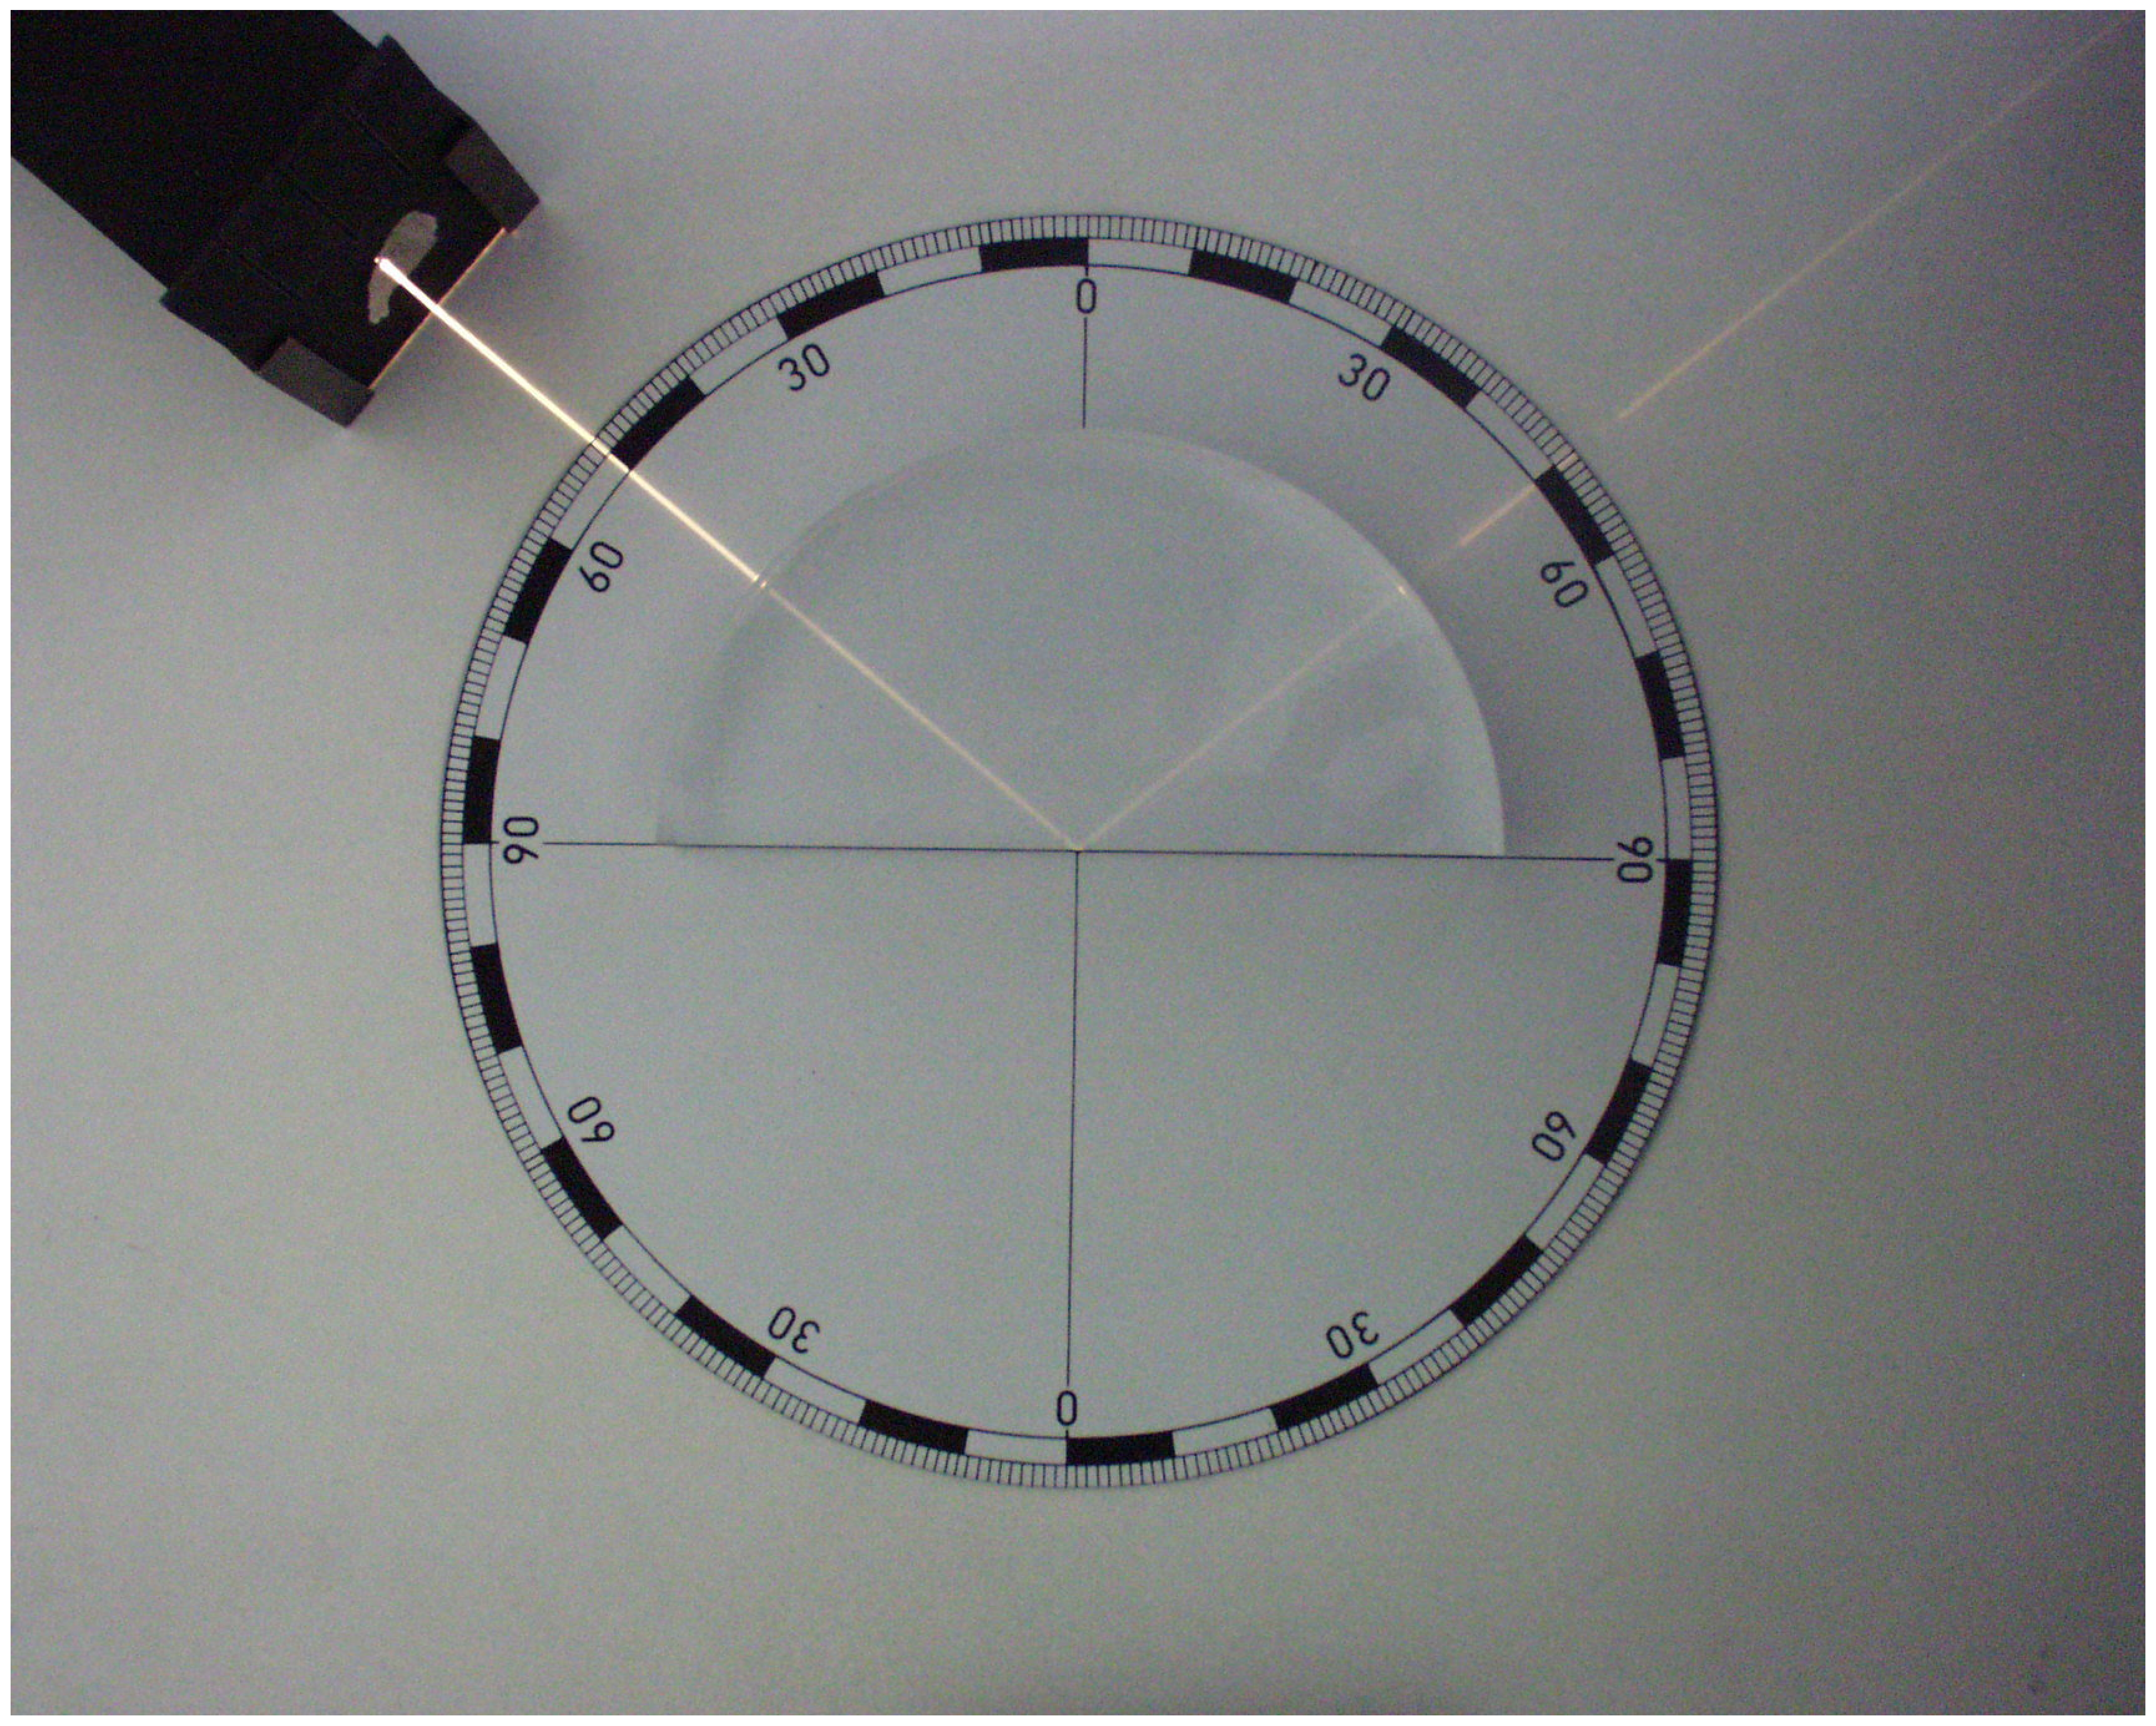
\includegraphics[width=\columnwidth]{modules/m0169_fTeljes_fenyvisszaverodes.eps} 
% https://en.wikipedia.org/wiki/File:Teljes_f%C3%A9nyvisszaver%C5%91d%C3%A9s.jpg
}}{A semicircle of glass is resting on the top half of a paper compass. The laser enters the convex side of the glass from the left at an angle of fifty degrees northwest from the vertical. Reflected wave is fifty degrees northeast. 
}
\end{center}
\centerline{\scriptsize 
\copyright~\hyperref[m0169_fTeljes_fenyvisszaverodes_Credit]{Z.\ S\'{a}ndor } 
\href{https://creativecommons.org/licenses/by-sa/3.0/}{CC BY-SA 3.0} 
} 
\caption{
\label{m0169_fTeljes_fenyvisszaverodes}
Total internal reflection of a light wave incident on a planar boundary between glass and air.
}
\end{figure}
%
\end{example}
%%%%%%%%%%%%%%%%%%%%%%%%%%%%%%%%%%%%%%%%%%%%%%%

Note also that the phase $\zeta$ of the reflection coefficient is precisely zero unless $\psi^i>\psi^i_c$, at which point it is both non-zero and varies with $\psi^i$.
This is known as the \emph{Goos-H{\"a}nchen effect}.
\index{Goos-H{\"a}nchen effect}
This leads to the startling phenomenon shown in Figure~\ref{m0169_fGHE}.
In this figure, the Goos-H{\"a}nchen phase shift is apparent as a displacement between the point of incidence and the point of reflection.  
%
\begin{figure}
\begin{center}
\pdftooltip{{  % note double braces
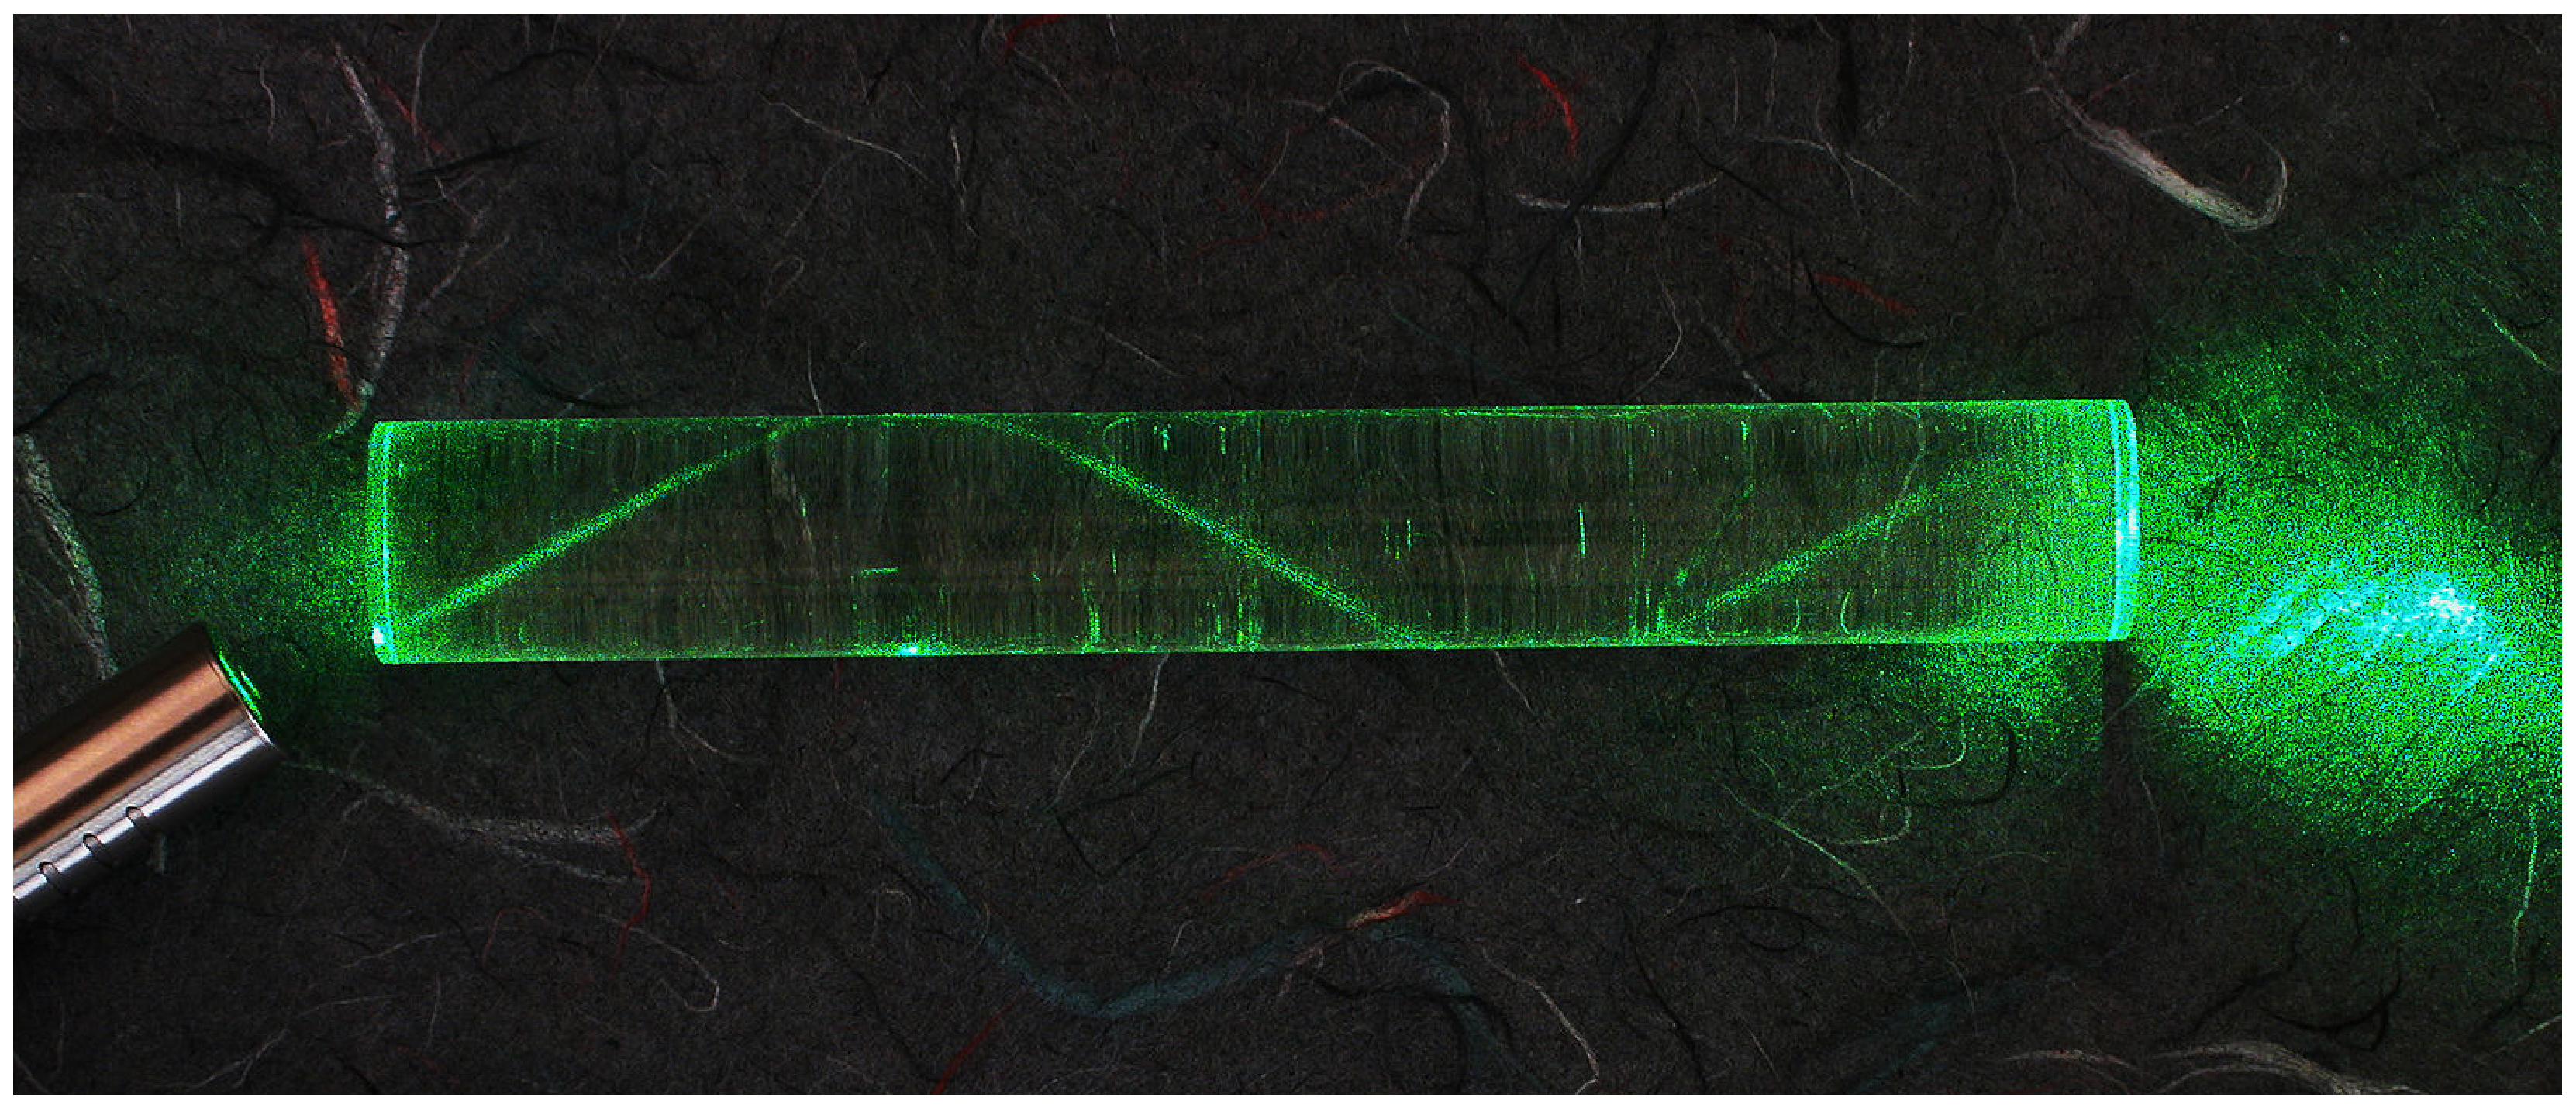
\includegraphics[width=\columnwidth]{modules/m0169_Laser_in_fibre.eps} 
% https://en.wikipedia.org/wiki/File:Laser_in_fibre.jpg
}}{Laser light travels through a rod at the bottom left and reflects off the internal surfaces of the rod creating a zigzag shape. Points of reflection appear to be displaced from points of incidence.}
\end{center}
\centerline{\scriptsize 
\copyright~\hyperref[m0169_fGHE_Credit]{Timwether} 
\href{https://creativecommons.org/licenses/by-sa/3.0/}{CC BY-SA 3.0} 
} 
\caption{
\label{m0169_fGHE}
Laser light in a dielectric rod exhibiting the Goos-H{\"a}nchen effect.  
}
\end{figure}

The presence of an imaginary component in the reflection coefficient is odd for two reasons.
First, we are not accustomed to seeing a complex-valued reflection coefficient emerge when the wave impedances of the associated media are real-valued.
Second, the \emph{total} reflection of the incident wave seems to contradict the boundary condition that requires the tangential components of the electric and magnetic fields to be continuous across the boundary.
That is, how can these components of the fields be continuous across the boundary if no power is transmitted across the boundary?
These considerations suggest that there \emph{is} a field on the opposite side of the boundary, but -- somehow -- it must have zero power.
This is exactly the case, as is explained in Section~\ref{m0170_Evanescent_Waves}.

%%%%%%%%%%%%%%%%%%%%%

{\bf Additional Reading:}
\begin{itemize}
\item ``\href{https://en.wikipedia.org/wiki/Goos%E2%80%93H%C3%A4nchen_effect}{Goos-H{\"a}nchen effect}'' on Wikipedia.
\item ``\href{https://en.wikipedia.org/wiki/Snell's_law}{Snell's law}'' on Wikipedia.
\item ``\href{https://en.wikipedia.org/wiki/Total_internal_reflection}{Total internal reflection}'' on Wikipedia.
\end{itemize}

\index{total internal reflection|)}

